% Name: Ellipse and its foci
% Description: The ellipse x²/a² + y²/b² = 1 with its semi-axes, its foci at distance c = √(a² − b²) from the center, and a point P whose distances to the foci add up to 2a.
% Tags: conic section, ellipse, foci, semi-axes

\usetikzlibrary{arrows.meta}

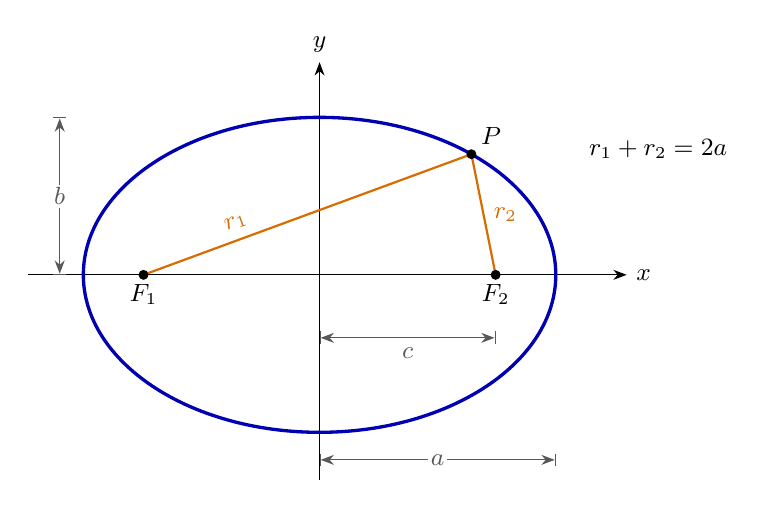
\begin{tikzpicture}[>={Stealth}, every node/.style={font=\small}]
  % a = 3, b = 2, so c = sqrt(5); P is the point at parameter 50 degrees, (3 cos 50, 2 sin 50)
  \pgfmathsetmacro{\c}{sqrt(5)}
  \coordinate (F1) at (-\c,0);
  \coordinate (F2) at (\c,0);
  \coordinate (P) at ({3*cos(50)},{2*sin(50)});
  \draw[->] (-3.7,0) -- (3.9,0) node[right] {$x$};
  \draw[->] (0,-2.6) -- (0,2.7) node[above] {$y$};
  \draw[very thick, blue!70!black] (0,0) ellipse (3 and 2);
  \draw[thick, orange!85!black] (F1) -- node[above, sloped, pos=0.3] {$r_1$} (P) -- node[right] {$r_2$} (F2);
  \draw[|<->|, gray!70!black] (0,-2.35) -- node[fill=white, inner sep=1pt] {$a$} (3,-2.35);
  \draw[|<->|, gray!70!black] (-3.3,0) -- node[fill=white, inner sep=1pt] {$b$} (-3.3,2);
  \draw[|<->|, gray!70!black] (0,-0.8) -- node[below] {$c$} (F2 |- 0,-0.8);
  \foreach \f/\n in {F1/{F_1}, F2/{F_2}} \fill (\f) circle (1.8pt) node[below] {$\n$};
  \fill (P) circle (1.8pt) node[above right] {$P$};
  \node[anchor=west] at (3.3,1.6) {$r_1 + r_2 = 2a$};
\end{tikzpicture}
